% --------------------------------------------------------------
% This is all preamble stuff that you don't have to worry about.
% Head down to where it says "Start here"
% --------------------------------------------------------------
 
\documentclass[12pt]{article}
\usepackage[margin=1in]{geometry} 
\usepackage{amsmath,amsthm,amssymb}
\usepackage{xcolor}
\usepackage{hyperref}
\hypersetup{
    colorlinks,
    citecolor=black,
    filecolor=black,
    linkcolor=black,
    urlcolor=blue
}
\newcommand{\code}{\texttt}
\setcounter{secnumdepth}{0}
\usepackage{graphicx}
\usepackage{epstopdf}
\usepackage{hyperref}
\epstopdfsetup{outdir=./}
\begin{document}
\title{\textbf{Compilers-II  (CS3423)}\\~\\Mini Assignment - I\\~\\An Introduction to the LLVM Infrastructure, AST, IR and Compiler Options}
\author{Sagar Jain\\CS17BTECH11034}
\maketitle
\begin{normalsize}
\tableofcontents
\end{normalsize}
\newpage
\section{Clang AST}
Clang is essentially a library that allows us to convert a  C program into an Abstract Syntax Tree and then manipulte the tree in some ways.
After viewing the ast for several non-trivial programs the following are a few observations:
\begin{enumerate}
\item The ast for any program can be printed using:\\ \code{clang -Xclang -ast-dump -fsyntax-only <filename>}. Here \code{Xclang} option is used to pass the arguments to the clang compiler, \code{fsyntax-only} is used so that no object code is generated and \code{ast-dump} is used to print the abstract syntax tree.
\item The dump begins with a bunch of \code{TypedefDecl} nodes followed by the ast for the user code.
\item We can use the option \code{ast-list} to get all a list of all the \textit{Declaration} nodes, this is an alternative option to look at the contents of the ast.
\item The \code{ast-view} option lets us look at an the entire ast graphically and is very easy to understand compared to the dump.Internally it creates a dot file which can be viewed by any dot file renderer. Example:
\begin{center}
\includegraphics[scale=0.6]{clangExamples/graph.eps}
\end{center}
\item We can also use clang-check to filter and print only the ast of a subset of the Declaration nodes:\\
\code{clang-check <filename> -ast-dump -ast-dump-filter=main --}
\end{enumerate}
\subsection{Observations about the AST structure}
\begin{itemize}
\item In the tree that clang creates, every node is an instance of one of the two classes: \textbf{Decl} or \textbf{Stmt} class. Nodes usually have a name followed by a type. For example, the main function begins with a \code{FunctionDecl} node which would have a name \textit{main} and a type(say \code{int} or \code{void}).
\item Functions start with \code{FunctionDecl} node which has the function name and type along with it. These are always followed by the \code{ParamVarDecl} nodes which have information about the function parameters and their types.
\item Most of the nodes in the body of the functions belongs to the Stmt class in the form of either of the following:
\begin{itemize}
\item CompoundStmt
\item DeclStmt
\item ImplicitCastExpr
\item CallExpr
\item ReturnStmt
\item Literals, etc.
\end{itemize}
\item Nodes like \code{ForStmt} have multiple children (5 for ForStmt) which are themselves nodes of different kind.
\item Nodes like \code{IntegerLiteral} contain the value of the node as well along with the type.
\end{itemize}
\newpage
\section{Clang AST Traversal}
The observations made about the AST traversal follows from this \href{http://clang.llvm.org/docs/RAVFrontendAction.html}{tutorial}.
\subsection{FrontendAction}
The class ASTFrontendAction is provided to us to be able to interact with the ast while compilation. We must create a class which inherits from FrontendAction to be able to execute user specific actions on the ast. We must implement a virtual method \code{CreateASTConsumer} in this class which returns a type of \code{std::unique\_ptr<clang::ASTConsumer>}, what we return is essentially our implementation of how we would like to consume the ast provided to us.
\subsection{ASTConsumer}
The clang class \code{ASTConsumer} is used to create the consumers for the ast. We must create a class that inherits from this class to be able to use the ast. We can have multiple different ways to enter the ast for example \code{HandleInlineFunctionDefinition}, \code{HandleTranslationUnit}, \code{HandleTopLevelDecl}, etc. We can override any of these methods to read the ast. This class must also have an implementation of RecursiveASTVisitor as its member, this implementation is defined in the following section. We can provide our consumer with \code{\&Compiler.getASTContext()} to give it information like source locations which are not stored in the ast nodes themselves.
\subsection{RecursiveASTVisitor}
We must implement a class which inherits from RecursiveASTVisitor to be used by the consumer class during the traversal. In this class we have methods of the type \code{VisitNodeType(NodeType *)} for different types of ast nodes. These methods return bool where \textit{true} implies that we want to continue the traversal and \textit{false} stops the traversal.
\newpage
\section{LLVM Error Messages}
\subsubsection{Programmatic Errors}
The observations on error messages have been made from \href{http://llvm.org/docs/ProgrammersManual.html}{here}.
In LLVM all the errors are classified into two types; \textit{programmatic} and \textit{recoverable}. Assertions are used heavily in the llvm-project. An assertion can be made to check if any code invariant or condition is being broken.\\
For example:\\
In \code{clang/lib/Analysis/CallGraph.cpp} we can find the following:\\
\hspace*{5ex} \code{assert(*CI != Root \&\& "No one can call the root node.")}
\\ We know that in a cfg there can be no calls to the root node, this assert is placed in the code to ensure this condition and also holds a message so that the user can know why the program has stopped execution.
\subsubsection{Recoverable Errors}
Recoverable errors are mostly the errors which occur because of reasons other than mistakes in the source code. These errors should be reported to the user as well. Reported errors are handled using the error scheme provided by LLVM. The error class can be used for any user defined errors and we can also specify information regarding the error in it. Template functions like \code{make\_error} are provided to construct failure values for the error class created by us which inherit from \code{ErrorInfo}.
\section{LLVM IR}
\section{Assembly Language}
\section{Compiler Toolchain}
\section{Kaleidoscope}
\end{document}